\documentclass[main.tex]{subfiles}
\begin{document}

%%%%%%%%%%%%%%%%%%%%%%%%%%%%%%%%%%%%%%%%%
%%%%%%%%%%% Tables of Results %%%%%%%%%%%
%%%%%%%%%%%%%%%%%%%%%%%%%%%%%%%%%%%%%%%%%
\subsection{Tables of Simulated Results}
% =========================================== 
\begin{figure}[H]
	\centering
	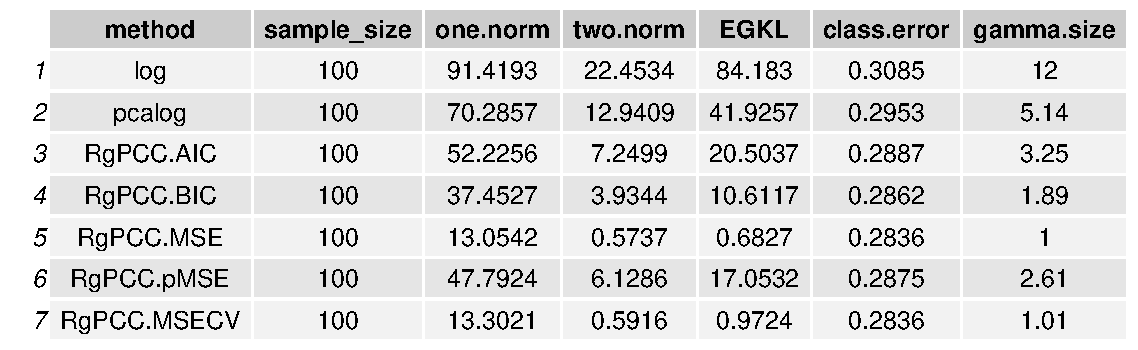
\includegraphics[width =  \textwidth]{simulated/(sparsity1-100,12)_metrics.pdf}
	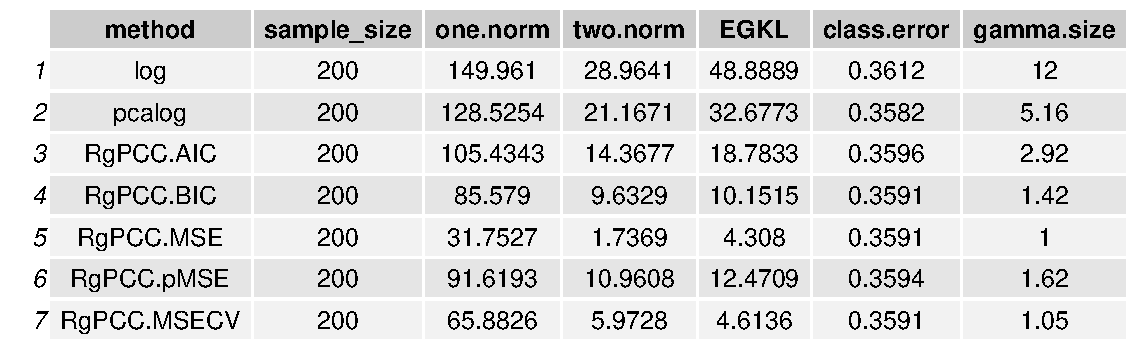
\includegraphics[width =  \textwidth]{simulated/(sparsity1-200,12)_metrics.pdf}
	\caption{Simulated results for RgPCC with parameters $\bgamma_1$ and $p = 12$.}
	\label{fig:simulated1-12}
\end{figure}

\begin{figure}[H]
	\centering
	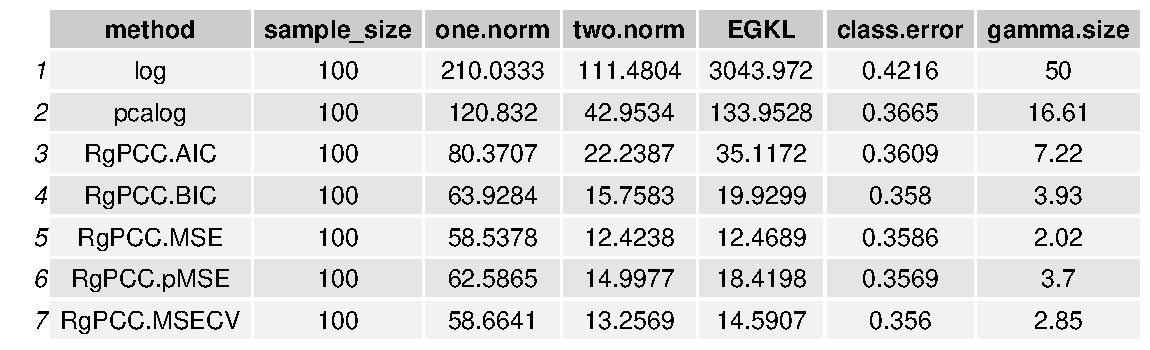
\includegraphics[width =  \textwidth]{simulated/(sparsity1-100,50)_metrics.pdf}
	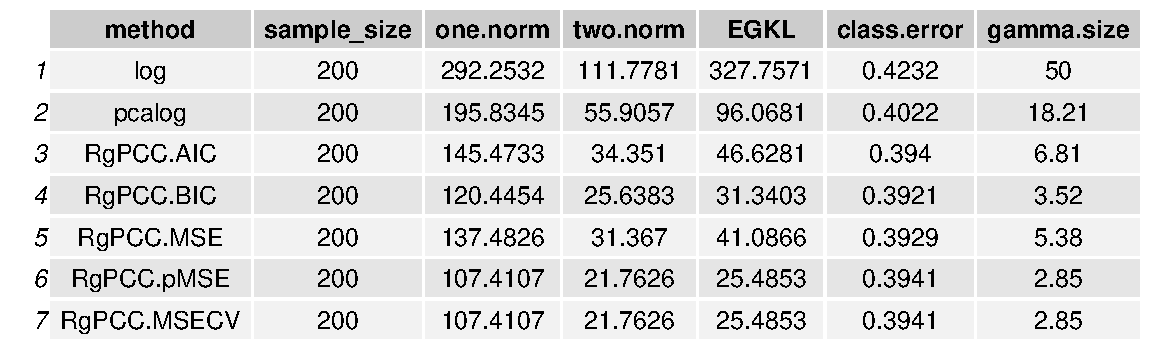
\includegraphics[width =  \textwidth]{simulated/(sparsity1-200,50)_metrics.pdf}
	\caption{Simulated results for RgPCC with parameters $\bgamma_1$ and $p = 50$.}
	\label{fig:simulated1-50}
\end{figure}

\begin{figure}[H]
	\centering
	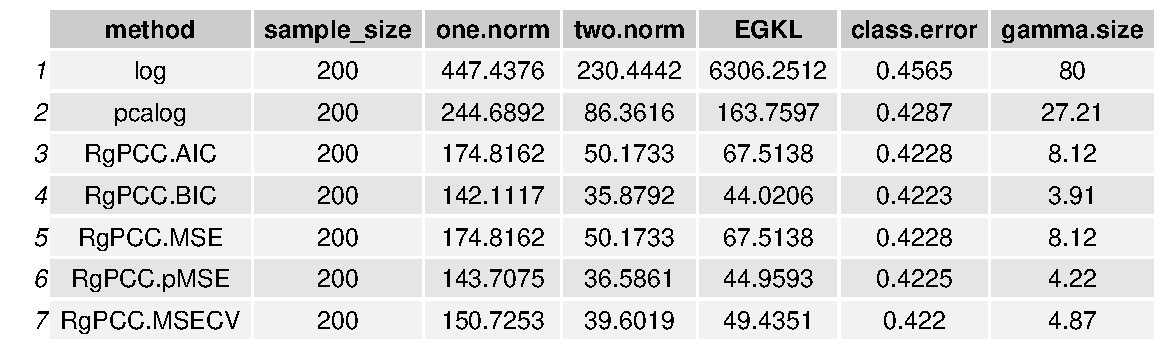
\includegraphics[width =  \textwidth]{simulated/(sparsity1-100,80)_metrics.pdf}
	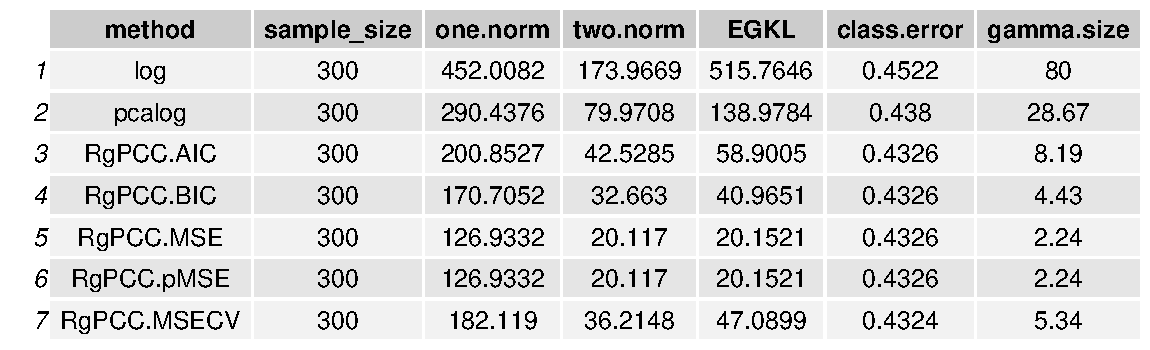
\includegraphics[width =  \textwidth]{simulated/(sparsity1-200,80)_metrics.pdf}
	\caption{Simulated results for RgPCC with parameters $\bgamma_1$ and $p = 80$.}
	\label{fig:simulated1-80}
\end{figure}

\begin{figure}[H]
	\centering
	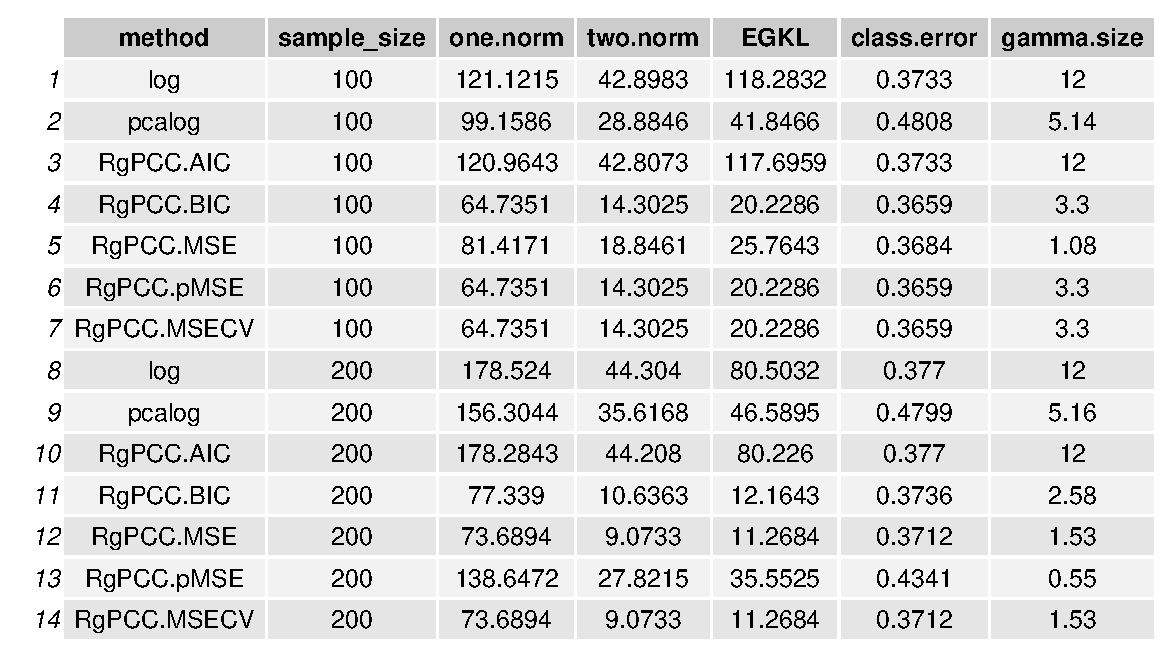
\includegraphics[width =  \textwidth]{simulated/(sparsity1-nonlead,12)_metrics.pdf}
	\caption{Simulated results for RgPCC with parameters $\bgamma_1'$ and $p = 12$.}
	\label{fig:simulated1-12-nonlead}
\end{figure}

\begin{figure}[H]
	\centering
	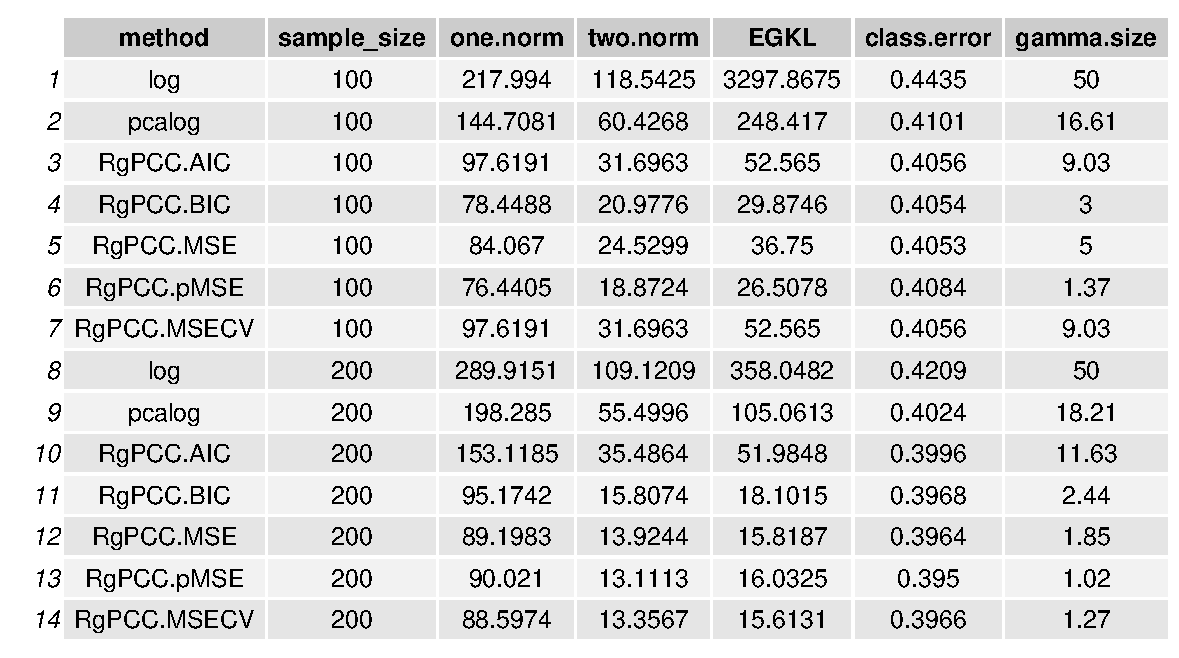
\includegraphics[width =  \textwidth]{simulated/(sparsity1-nonlead,50)_metrics.pdf}
	\caption{Simulated results for RgPCC with parameters $\bgamma_1'$ and $p = 50$.}
	\label{fig:simulated1-50-nonlead}
\end{figure}

\begin{figure}[H]
	\centering
	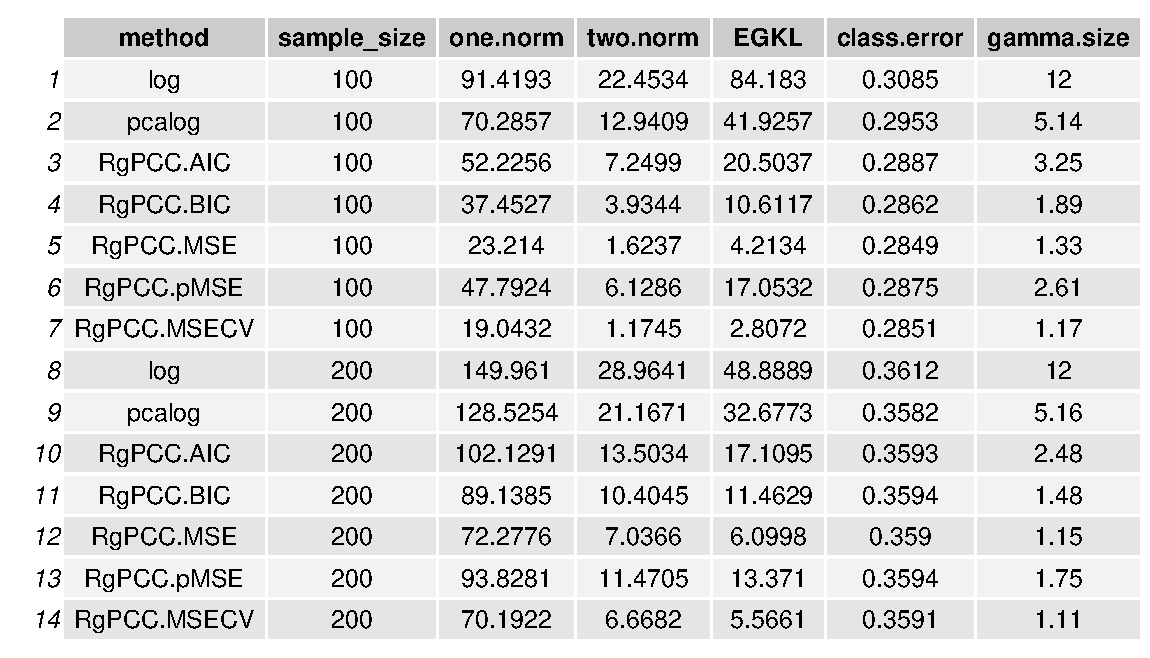
\includegraphics[width =  \textwidth]{simulated/(sparsity3,12)_metrics.pdf}
	\caption{Simulated results for RgPCC with parameters $\bgamma_2$ and $p = 12$.}
	\label{fig:simulated3-12}
\end{figure}

\begin{figure}[H]
	\centering
	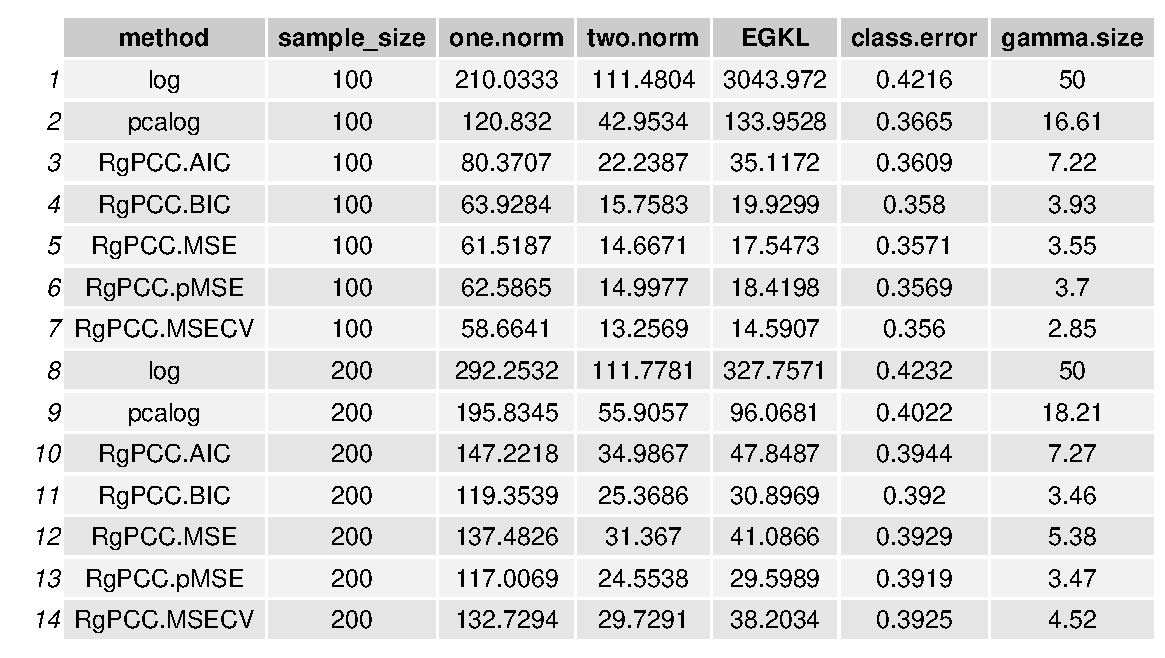
\includegraphics[width =  \textwidth]{simulated/(sparsity3,50)_metrics.pdf}
	\caption{Simulated results for RgPCC with parameters $\bgamma_2$ and $p = 50$.}
	\label{fig:simulated3-50}
\end{figure}

\begin{figure}[H]
	\centering
	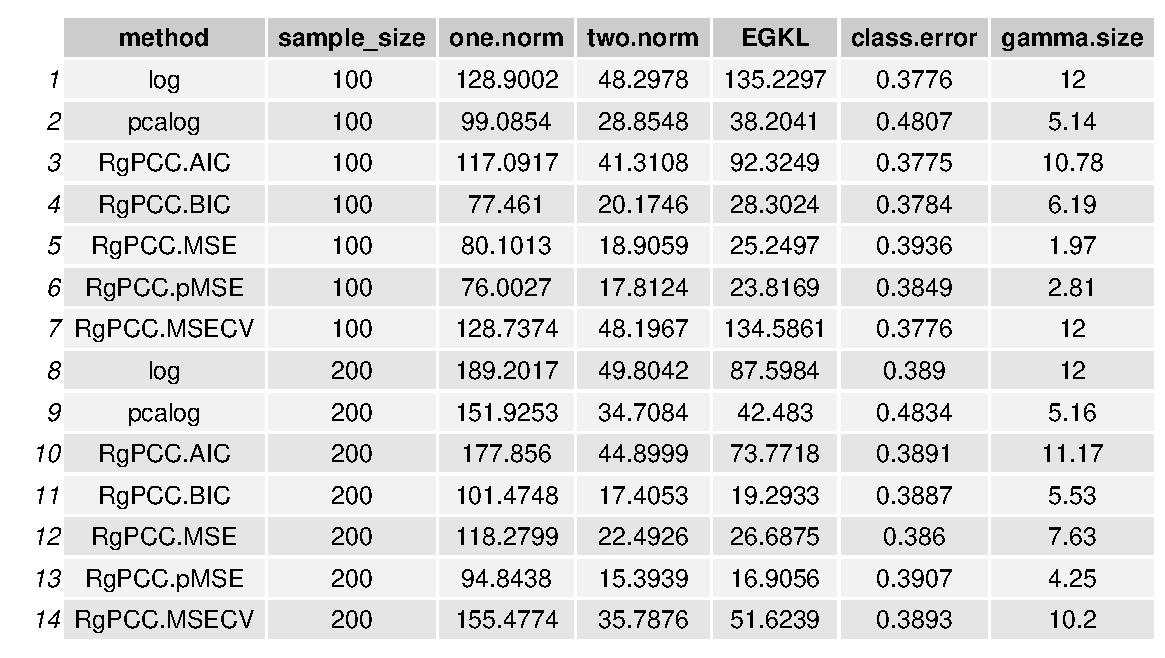
\includegraphics[width =  \textwidth]{simulated/(sparsity3-nonlead,12)_metrics.pdf}
	\caption{Simulated results for RgPCC with parameters $\bgamma_2'$ and $p = 12$.}
	\label{fig:simulated3-12-nonlead}
\end{figure}

\begin{figure}[H]
	\centering
	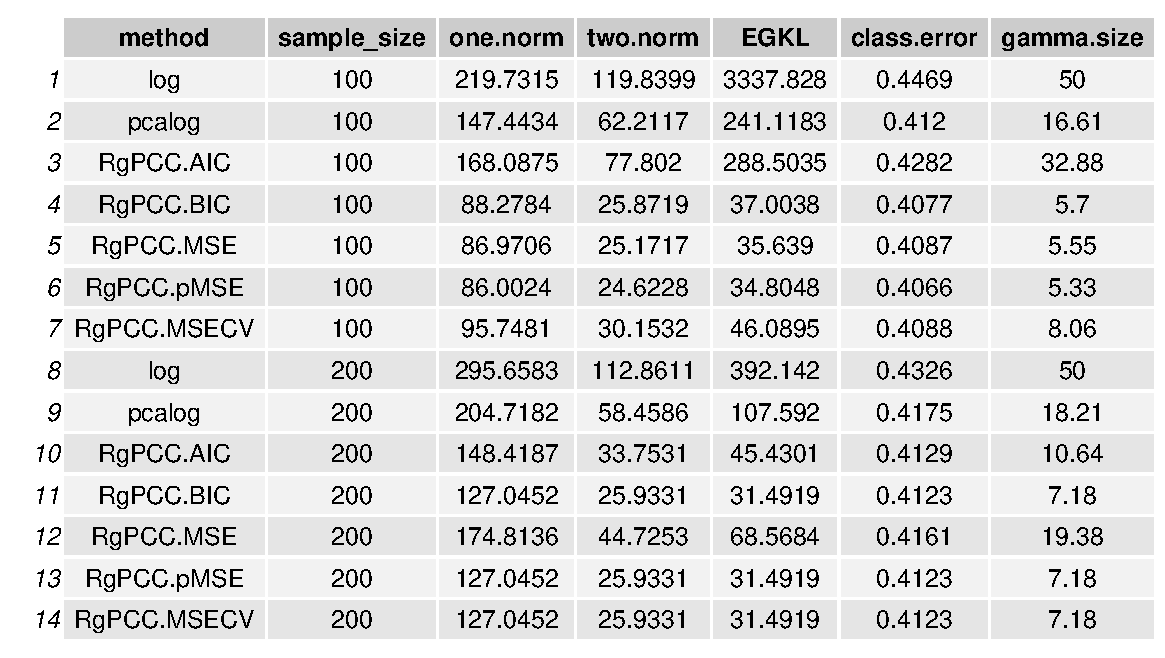
\includegraphics[width =  \textwidth]{simulated/(sparsity3-nonlead,50)_metrics.pdf}
	\caption{Simulated results for RgPCC with parameters $\bgamma_2'$ and $p = 50$.}
	\label{fig:simulated3-50-nonlead}
\end{figure}

\begin{figure}[H]
	\centering
	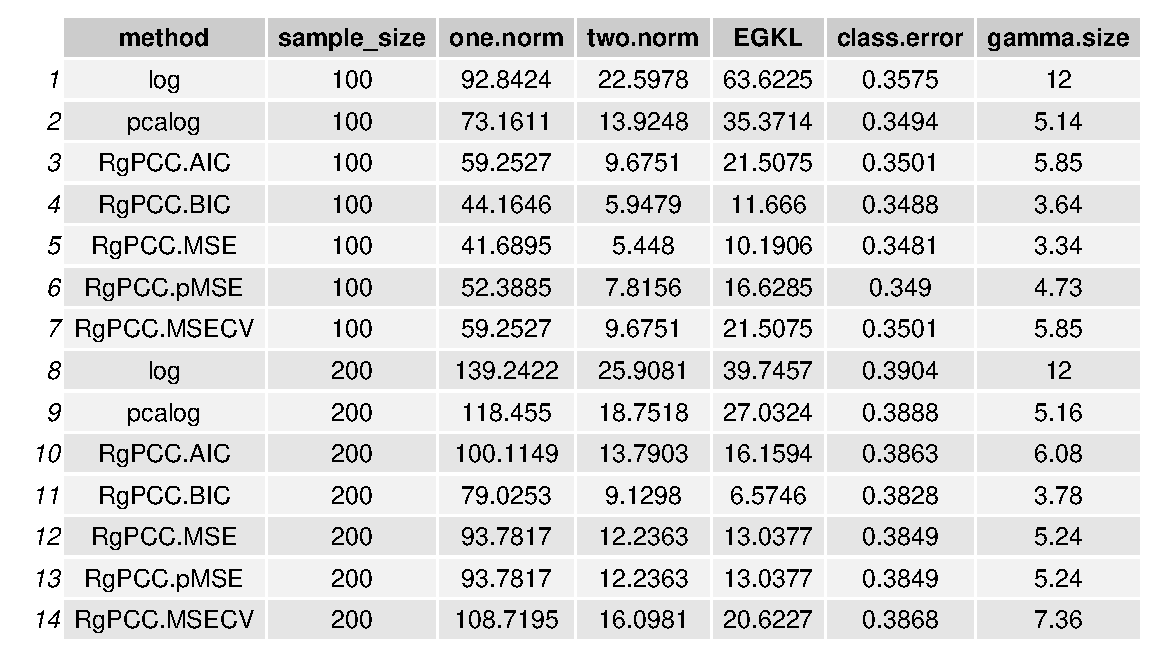
\includegraphics[width =  \textwidth]{simulated/(sparsity5,12)_metrics.pdf}
	\caption{Simulated results for RgPCC with parameters $\bgamma_3$ and $p = 12$.}
	\label{fig:simulated5-12}
\end{figure}

\begin{figure}[H]
	\centering
	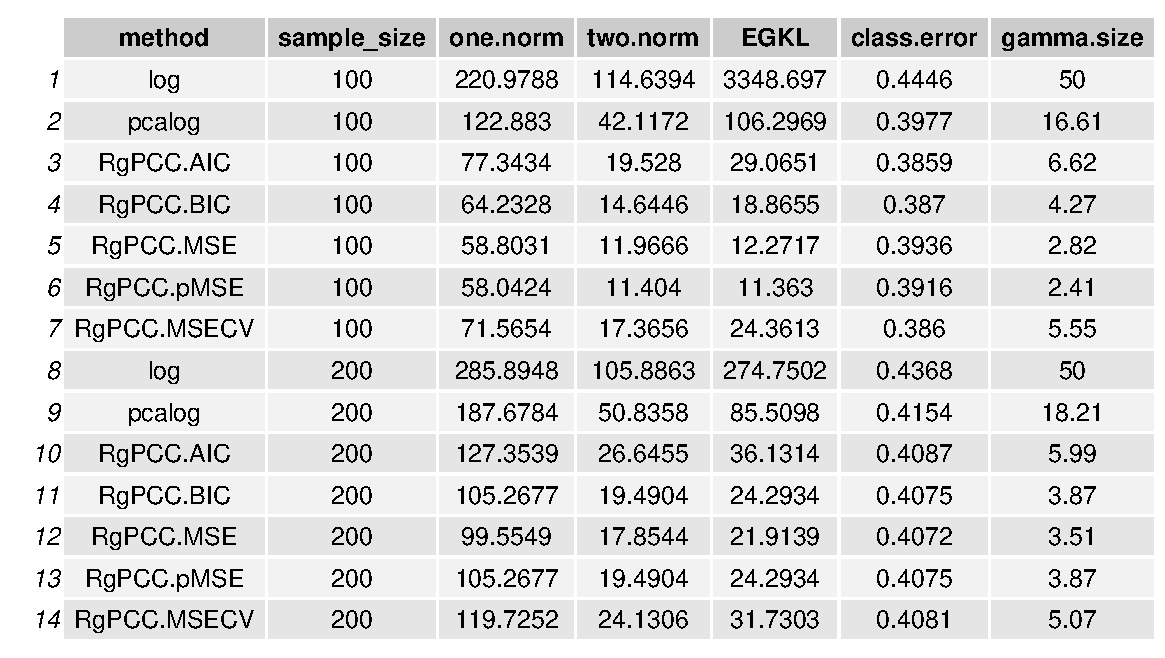
\includegraphics[width =  \textwidth]{simulated/(sparsity5,50)_metrics.pdf}
	\caption{Simulated results for RgPCC with parameters $\bgamma_3$ and $p = 50$.}
	\label{fig:simulated5-50}
\end{figure}

\begin{figure}[H]
	\centering
	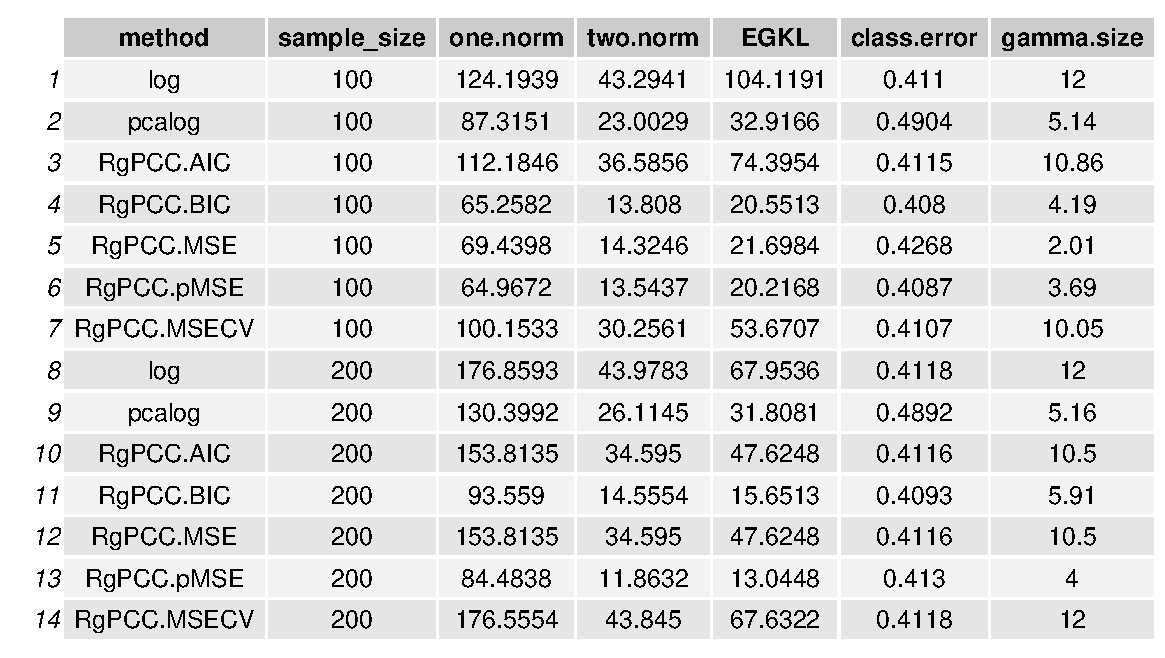
\includegraphics[width =  \textwidth]{simulated/(sparsity5-nonlead,12)_metrics.pdf}
	\caption{Simulated results for RgPCC with parameters $\bgamma_3'$ and $p = 12$.}
	\label{fig:simulated5-12-nonlead}
\end{figure}

\subsection{Graphs of Tuning}

\end{document}